%
% This is the LaTeX template file for lecture notes for EE 382C/EE 361C.
%
% To familiarize yourself with this template, the body contains
% some examples of its use.  Look them over.  Then you can
% run LaTeX on this file.  After you have LaTeXed this file then
% you can look over the result either by printing it out with
% dvips or using xdvi.
%
% This template is based on the template for Prof. Sinclair's CS 270.

\documentclass[twoside]{article}
\usepackage{graphics}
\setlength{\oddsidemargin}{0.25 in}
\setlength{\evensidemargin}{-0.25 in}
\setlength{\topmargin}{-0.6 in}
\setlength{\textwidth}{6.5 in}
\setlength{\textheight}{8.5 in}
\setlength{\headsep}{0.75 in}
\setlength{\parindent}{0 in}
\setlength{\parskip}{0.1 in}

%
% The following commands set up the lecnum (lecture number)
% counter and make various numbering schemes work relative
% to the lecture number.
%
\newcounter{lecnum}
\renewcommand{\thepage}{\thelecnum-\arabic{page}}
\renewcommand{\thesection}{\thelecnum.\arabic{section}}
\renewcommand{\theequation}{\thelecnum.\arabic{equation}}
\renewcommand{\thefigure}{\thelecnum.\arabic{figure}}
\renewcommand{\thetable}{\thelecnum.\arabic{table}}

%
% The following macro is used to generate the header.
%
\newcommand{\lecture}[4]{
   \pagestyle{myheadings}
   \thispagestyle{plain}
   \newpage
   \setcounter{lecnum}{#1}
   \setcounter{page}{1}
   \noindent
   \begin{center}
   \framebox{
      \vbox{\vspace{2mm}
    \hbox to 6.28in { {\bf EE 382V: Social Computing
                        \hfill Fall 2018} }
       \vspace{4mm}
       \hbox to 6.28in { {\Large \hfill Homework #1: #2  \hfill} }
       \vspace{2mm}
       \hbox to 6.28in { {\it Partner1: #3 \hfill Partner2: #4} }
      \vspace{2mm}}
   }
   \end{center}
   \markboth{EE382V:Social Computing HW#1: #2}{EE382V:Social Computing HW#1: #2}
   %{\bf Disclaimer}: {\it These notes have not been subjected to the
   %usual scrutiny reserved for formal publications.  They may be distributed
   %outside this class only with the permission of the Instructor.}
   \vspace*{4mm}
}

%
% Convention for citations is authors' initials followed by the year.
% For example, to cite a paper by Leighton and Maggs you would type
% \cite{LM89}, and to cite a paper by Strassen you would type \cite{S69}.
% (To avoid bibliography problems, for now we redefine the \cite command.)
% Also commands that create a suitable format for the reference list.
\renewcommand{\cite}[1]{[#1]}
\def\beginrefs{\begin{list}%
        {[\arabic{equation}]}{\usecounter{equation}
         \setlength{\leftmargin}{2.0truecm}\setlength{\labelsep}{0.4truecm}%
         \setlength{\labelwidth}{1.6truecm}}}
\def\endrefs{\end{list}}
\def\bibentry#1{\item[\hbox{[#1]}]}

%Use this command for a figure; it puts a figure in wherever you want it.
%usage: \fig{NUMBER}{SPACE-IN-INCHES}{CAPTION}
\newcommand{\fig}[3]{
			\vspace{#2}
			\begin{center}
			Figure \thelecnum.#1:~#3
			\end{center}
	}
% Use these for theorems, lemmas, proofs, etc.
\newtheorem{theorem}{Theorem}[lecnum]
\newtheorem{lemma}[theorem]{Lemma}
\newtheorem{proposition}[theorem]{Proposition}
\newtheorem{claim}[theorem]{Claim}
\newtheorem{corollary}[theorem]{Corollary}
\newtheorem{definition}[theorem]{Definition}
\newenvironment{proof}{{\bf Proof:}}{\hfill\rule{2mm}{2mm}}

% **** IF YOU WANT TO DEFINE ADDITIONAL MACROS FOR YOURSELF, PUT THEM HERE:

\begin{document}
%FILL IN THE RIGHT INFO.
%\lecture{**LECTURE-NUMBER**}{**DATE**}{**LECTURER**}{**SCRIBE**}
\lecture{1}{September 25}{Javier Palomares}{Porter Perry}
%\footnotetext{These notes are partially based on those of Nigel Mansell.}

% **** YOUR NOTES GO HERE:

% Some general latex examples and examples making use of the
% macros follow.  
%**** IN GENERAL, BE BRIEF. LONG SCRIBE NOTES, NO MATTER HOW WELL WRITTEN,
%**** ARE NEVER READ BY ANYBODY.
\section{Question1}
Consider a bipartite graph with a set of boys and girls [and the number of boys is equal to the number of girls]. Suppose that every girl likes at least $d \geq 1$ boys and every boy likes at most $d$ girls. Show that there exists a perfect matching between boys and girls.

\subsection{Answer1}
According to Hall’s [Marriage] theorem, if there no constricted set, then a perfect matching exists. 

Let the set A represent the set of girls, and set B represent the set of boys. 

Assume that there is a subset $S \subseteq A$, and it’s set of neighbors in the set of boys $N(S)$, such that it forms a constricted set where $|S| > |N(S)|$. 

Let $d_{1}$ be the minimum degree of any girl, and $d_{2}$ be the maximum degree of any boy. Then, $d_{1} \geq d$ and $d_{2} \leq d$, so $d_{1} \geq d_{2}$.

Let $D(S)$ be the sum of the degree of nodes within the subset S. Then $d_{1}|S| \leq D(S)$, since every girl node of $S$ has a degree of at least $d_{1}$. 
Likewise, $d_{2}|N(S)| \geq D(S)$, since every boy node in $N(S)$ has a degree of at most $d2$ edges.

So,\\[16pt]
$d_{1}|S| \leq  D(S) \leq d2|N(S)|$

$d_{1}|S| \leq  d2|N(S)|$

$|S| \leq  \frac{d_{2}}{d_{1}}|N(S)| $\\[16pt]
Since $d_{1} \leq d_{2}$, $|S| \leq |N(S)|$, which contradicts $S$ and $N(S)$ being a constricted set.\\[8pt]
Thus, by Hall’s [Marriage] Theorem, a perfect matching exists. 


\newpage
\section{Question2}
Show that K\"{o}nig--Egerváry Theorem implies Hall’s Theorem. 

\subsection{Answer2}

Hall’s [Marriage] theorem states that if there is no constricted set, then a perfect matching exists. 

The K\"{o}nig--Egerváry theorem states that in any bipartite graph, the number of edges in a maximum matching is equal to the number of vertices in a minimum vertex cover.\\[12pt]

\textbf{Proof:} No constricted set implies a perfect matching exists (by contradiction).

Let there be bipartite graph $G=(A, B, E)$ that consists of  two partitioned sets $A$ and $B$ of vertices and a set $E$ or edges between the two. Let $M$ represent the set of maximum matching edges and $V$ represent the minimum vertex cover.

Assume that there is no constricted set and no perfect matching. Then the maximum matching size $m < |A|$. By the K\"{o}nig--Egerváry theorem, the minimum vertex cover also has size $m < |A|$.

Let $X = A \cap V$ and $Y = B \cap V$.  Since the set $V$ is a vertex cover on ${A, B}$, then 
$|X| + |Y| = |V| = m < |A|$.

Rearranging this, $|Y| < |A| - |X| = |A - X|$.
Also, since $V$ is a vertex cover, then there are no edges between $A - X$ and $B - Y$.

So $N(A - X) \leq |Y| < |A - X|$, which is a constricted set and contradicts our assumption. Therefore a perfect matching must exist.\\[12pt]

\textbf{Proof:} A perfect matching exists implies no constricted set.

If a perfect matching exists, then any set $S \subseteq A$ is matched to $|S|$ vertices in $B$. 

So, $\forall S \subseteq A$, $|N(S)|=|S|$, so no constricted set exists.
 

\newpage
\section{Question3}
An $r \times n$ Sudoku is an $r \times n$ matrix with entries ${1, \ldots ,n}$ such that each number appears at most once in each row and column. Show that any $r \times n$ Sudoku can be extended to an $(r+1) \times n$ Sudoku whenever $r < n$.

\subsection{Answer3}
Proof by induction.

Base case $(r=1)$. Show that a $1 \times n$ Sudoku can be extended to $2 \times n$ for $n > 1$.
One way to extend is to copy row 1 of any $1 \times n$ Sudoku and insert it into row 2, but shift every element in the row by 1, so that the element at column $i$ in row 1 is at column $(i + 1) \% n$. 

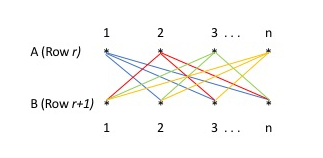
\includegraphics{SudokuFigure1}
 
We have a bipartite graph $G=(A, B, E)$ where $A={1, 2 , 3, \ldots n}$, $B={1, 2, 3, \ldots n}$, and edges $e_{ij} \in E$ that connect $i \in A$ to $j \in B$ where the $i^{th}$ column of the Sudoku does not have the number $j$. If there is a perfect matching on $G$, we can extend the Sudoku by a row, as long as the number of resultant rows is less than or equal to $n$. 

To do this, take the matching $(i,j)$ of the perfect matching and place $j$ on row $r+1$ at column $i$.\\[12pt]

\textbf{Proof} that a perfect matching exists:

First, note that in a Sudoku with $r$ rows, column $i$ has $r$ distinct numbers in it. Therefore, column $i$ has $(n - r)$ edges to the $(n - r)$ numbers not in column $i$. Then every element $j \in B$ appears exactly once in each row and at most once in any of the $n$ columns, so there are $(n - r)$ column where $i$ can be placed. 

Thus, every element $j \in B$ is adjacent to $(n - r)$ edges, and a perfect matching exists.

\end{document}





